\taughtsession{Lecture}{Names, Bindings, Scopes and Memory Allocation}{2024-03-11}{1400}{Jiacheng}{}


\section{Variables \& Attributes}
A \textit{Variable} is a place holder (a named memory location) for a value at run-time. Variables have several attributes at run-time which includes:
\begin{description}
    \item[name] which provides the means for accessing a variable
    \item[address] (also known as it's l-value) which is what is required when the name of the variable appears in the left side of an assignment 
    \item[value] which is the contents of the memory cell(s) (also known as the r-value of a variable)
    \item[type] which determines the range of values that the variable can store and the operations that are defined for the values
    \item[lifetime] which defines the time during which a variable is bound to a specific memory location (i.e. it's address) 
    \item[scope] which is the range of statement in which the variable is visible / accessible 
\end{description}

\section{Declaration}
In most languages, variables are introduced using a declaration. This can either be done implicitly or explicitly.
\subsection{Explicit Declaration}
An Explicit Declaration is a program statement used for declaring the type of the variable. For example, a variable, \verb|i|, is declared in different languages as follows:
\begin{itemize}
    \item in Pascal \verb|i : integer|
    \item in Java \verb|int i;|
    \item in Fortran \verb|INTEGER :: Count|
\end{itemize}
\subsection{Implicit Declaration}
An implicit declaration is a default mechanism for specifying types of variables through default conventions rather than declaration statements. For example, Fortran has both explicit and implicit declarations:
\begin{description}
    \item[Explicit]\ 
    \begin{verbatim}
    INTEGER :: Count, Total
    REAL :: Average, Sum
    COMPLEX :: c
    \end{verbatim}
    \item[Implicit] The default implicit typing rule is that if the first letter of the name is \verb|I|, \verb|J|, \verb|K|, \verb|L|, \verb|M|, or \verb|N|, then the data type is integer, otherwise it's real.
\end{description}
\subsection{Type Inference}
Another kind of implicit type declaration is type inference. This is popular in \textit{modern, edgy} language such as JavaScript and C\# whereby a variable can be declared with \verb|var| or \verb|let| and set with an initial value. This initial value sets the type of the variable. Python takes this one step further whereby a variable is just defined. That's it, there is no keyword required to say that you're defining a variable. For this to work, an initial value must be provided.\\

Type Inference (a way to declare a type) is different from reference type (a data type, e.g. pointer type)

\section{Binding}
A binding is an association between an entity and an attribute, for example - between a variable and it's type, or value, or memory location; or between a symbol (e.g. \verb|+|) and an operation.\\

Binding time is the time at which a binding takes place, which can be at different times. 

\subsection{Binding Time}
If we take the following Java Statements:
\begin{verbatim}
    int count;
    count = count + 5;
\end{verbatim}
We can then review the attributes of the statements and when they're bound.
\begin{description}
    \item[type] of \verb|count| is at \textit{compile time} (because is a typed language, a variable must be declared before it's used)
    \item[range] of possible values of \verb|count| is bound at \textit{compiler design time} 
    \item[operation] (the meaning) of the operator \verb|+| is bound at \textit{compile time} when the types of its operands have been determined
    \item[value] of \verb|count| is bound at the execution of the statement, i.e. \textit{runtime}
\end{description}

It is also possible for binding to take place at load time or link time.
\begin{description}
    \item[Load time] whereby we are binding a C or C++ \verb|static| variable to a memory location
    \item[Link time] whereby we are binding the variables in one module with those in another
\end{description}

\subsection{Type Binding: Static vs Dynamic}
A type binding is static if it occurs before runtime and remains unchanged throughout program execution. For example, declarations (implicit or explicit) always carry the type information, and binding is done at compile time. Languages which conform to this are said to be statically typed and include Java, C, Fortran, Pascal, etc. It is advantageous to use one because they are more efficient and the type errors can be detected by the compiler. However, they are disadvantageous because they're not very flexible for interactive applications.\\

Languages which complete type-binding during execution, or where they can change during execution of the program (specified through an assignment statement) use \textit{dynamic} type binding. Examples of languages which do this include Python, JavaScript and PHP. It is advantageous to use a dynamically typed language as they have greater flexibility (given the possibility to produce generic program units); and allow for rapid prototyping. However they are disadvantageous as they have a higher resource cost (given the dynamic type checking at run-time); and that the type-error detection by the compiler is difficult.

\subsection{Strong vs Weak Typing}
Languages in which all the type errors (where the use of an operator to an operand of an inappropriate type) can be detected by the compiler, that language is known as \textit{type safe}. For example, Java, Haskell and Ada are type safe; however FORTRAN and C are not. Type safe languages are said to be \textit{strongly typed}. Strongly typed languages can either be static of dynamic typed.\\

Languages which aren't type safe are said to be \textit{weakly typed}. Dynamic Typed does not necessarily mean weakly typed, for example Python's typing is dynamic but it is strongly typed.\\

Some languages as a whole are not typed safe, however they might have a subset of instructions that are type safe - for example Mesa for Systems Programming.

\begin{figure}[H]
    \centering

    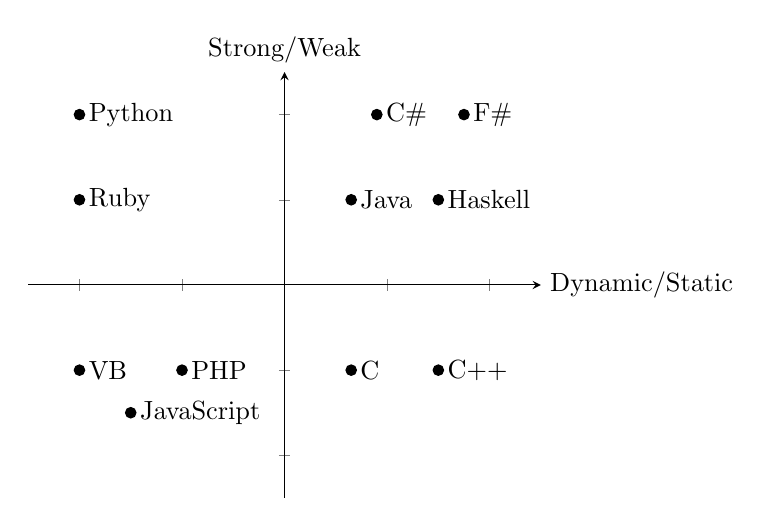
\begin{tikzpicture}[scale=0.95]
    \begin{axis}[%axis equal=true,
        axis y line=center, 
        axis x line=middle, 
        axis on top=true,
        xmin=-5, xmax=5, 
        ymin=-5, ymax=5,
        yticklabel=\empty,
        xticklabel=\empty,
        xlabel={Dynamic/Static},
        x label style={at={(axis description cs:1,0.5)},anchor=west},
        ylabel={Strong/Weak},
        y label style={at={(axis description cs:0.5,1)},anchor=south},
    ] 
    \draw [black, fill] (-4,4) circle (2pt) node [right] {Python};
    \draw [black, fill] (-4,2) circle (2pt) node [right] {Ruby};
    \draw [black, fill] (-4,-2) circle (2pt) node [right] {VB};
    \draw [black, fill] (-2,-2) circle (2pt) node [right] {PHP};
    \draw [black, fill] (-3,-3) circle (2pt) node [right] {JavaScript};
    \draw [black, fill] (1.3,-2) circle (2pt) node [right] {C};
    \draw [black, fill] (3,-2) circle (2pt) node [right] {C++};
    \draw [black, fill] (3,2) circle (2pt) node [right] {Haskell};
    \draw [black, fill] (1.3,2) circle (2pt) node [right] {Java};
    \draw [black, fill] (3.5,4) circle (2pt) node [right] {F\#};
    \draw [black, fill] (1.8,4) circle (2pt) node [right] {C\#};    
    \end{axis} 
    \end{tikzpicture} 
    
    \caption{Strong-Weak vs Dynamic-Static Language Typing}
\end{figure}

\section{Block Structure of Programs}
Modern programming languages use \textit{blocks}. These are subsections of code which have a specific purpose and they define a local reference environment which is useful in relation to variable binding \& scope. Blocks are denoted by start and end markers, in sensible languages (such as C, C++, Java) this is braces (\verb|{| and \verb|}|); however in silly languages such as Python, this is through indentation. \\

A block can contain declaration of variables local to that region and have its own \textit{reference environment} (the accessible names / identifiers)

\subsection{Nesting Blocks}
Blocks are typically nested. This is seen in Java and C in that method blocks are always nested within class blocks and other code blocks can be nested within these. However in Java and C, it is not possible to nest methods within methods. We can also see nesting blocks in Python and pascal, where procedures (which have no return value) and functions (which have a return value) can be nested.\\

When designing an algorithm, we have to consider the local reference environment to decide the scope identifiers in name resolution. This involves considering: where these identifiers can be used / accessed; and what happens if we have two identifiers which have the same name.

\section{Scope of Identifiers}
The scope of an identifier (e.g. a variable or a procedure) is the part of the program text that can access the identifer. If we take the following Pascal program as an example:
\begin{verbatim}
    program my_prog;
    var
        i, j : integer;
    procedure f (k : integer);
    var
        j : integer;
    begin
        j := k + i;
    end
    procedure g (k : integer);
    begin
        f(k+1);
    end
    begin
        i := 5; j := 3; g(j);
    end.
\end{verbatim}
In most languages, an identifiers scope is the block in which it's declared. For example, in the above program:
\begin{itemize}
    \item the variables, \verb|i|, \verb|j| declared in the outermost block are \textit{global variables} (their scope is the whole program)
    \item the scope of parameter \verb|k| and local variable \verb|j| is the body of procedure \verb|f|. The use of variable \verb|j| (in the body of \verb|f|) is bound to its local declaration (not the \verb|j| that has been globally declared)
    \item procedures \verb|f| and \verb|g| are declared in the outermost block and are therefore global
\end{itemize}
\subsection{Visibility Rules for Duplicated Identifiers}
A declaration in an inner block hides a declaration of a variable in an enclosing block with the same name - this \textit{visibility rule} is adopted by most languages within blocks.\\

Using the example above - the local variable \verb|j| in procedure \verb|f| hides the global variable \verb|j|. Where this is the case - we say that there is \textit{a hole in the scope} of the global variable \verb|j| (as its scope is the whole program except procedure \verb|f|).

\subsection{Static and Dynamic Scoping}
In the Pascal program above, the scopes of variables are governed by the visibility rules. Therefore the scopes of variables depend on the lexical structure (the layout) of the program which means that it is possible for a compiler to determine the scopes of all variables. This is known as \textit{static} or \textit{lexical}
scoping. \\

By contrast, \textit{dynamic scoping} is where the reference environment (the visibility of identifiers) depends on the calling sequence of subprograms, not the layout of the nesting structures. Therefore the scopes of identifiers can be determined only at runtime. \\

Dynamic scoping is not popular: it gives less-reliable programs because subprograms are always executed in the environment of all previously called subprograms that have not yet completed their execution. Dynamic scoping also leads to programs of poor readability. However, it is easier to implement using stacks and resolving a variable does not require tracing the syntactic structure of the entire program. Dynamic Scoping was used by early versions of LISP and is still in operation in Perl and Common LISP. 

\subsubsection{An Example}
If we consider the following pseudocode (based on JavaScript syntax) function, \verb|big|, in which two functions \verb|sub1| and \verb|sub2| are nested:
\begin{verbatim}
    function big(){
        function sub1(){
            var x = 7;
            sub2();
        }
        function sub2(){
            var y = x;
        }
        var x = 3;
        sub1();
    }
\end{verbatim}

The \verb|x| which is referenced within \verb|sub2()| depends on the scoping type.\\

\textbf{In Static Scoping}
\begin{itemize}
    \item When resolving the identifier \verb|x|, the search for \verb|x| begins in the body of function \verb|sub2()|. Here it is found that there is a reference for \verb|x|, but no declaration for \verb|x| is found.
    \item With static scoping, the search continues to the static parent of \verb|sub2()| (the function \verb|big()|), in which \verb|x| is declared (in the line \verb|var x = 3;|).
    \item If there is no declaration of \verb|x| in \verb|big()|, then an error is generated. The \verb|x| declared in \verb|sub1()| is ignored. 
\end{itemize}

\textbf{In Dynamic Scoping}
\begin{itemize}
    \item The process of resolving \verb|x| in \verb|sub2()| depends on the calling sequence of the functions. This cannot be determined at compile time.
    \item In this case, the searching for \verb|x| also begins in the body of \verb|sub2()|, where no declaration for \verb|x| is found.
    \item After that, the search for \verb|x| is rather different to static scoping - in that the call stack is searched until a declaration of \verb|x| is located. In the above example, the search for \verb|x| begins in \verb|sub2()|, then moves to it's caller (also known as it's dynamic parent) \verb|sub1()|, where \verb|x| is declared (with the line \verb|x = 7;|) and therefore is found. The value of \verb|x| is then assigned to \verb|y|
\end{itemize}

\section{Lifetime of Variables}
The \textit{lifetime} of a variable is the period in which it ``exists'' and has a value assigned to it during the given program execution. For local variables within procedures, the lifetime is the current execution of the procedure; which means the variable is created when the procedure is called and destroyed when the procedure exits. Each (recursive) execution of a procedure has its own copy of the local variables. The lifetime of a global variable is the entire duration of the execution of the program. 

\subsection{Lifetime and Memory Allocation}
The lifetime of a name / variable is related to how memory is allocated and deallocated for its values. There are three basic \textit{memory allocation mechanisms}, each associated with a different area of memory.
\begin{description}
    \item[static allocation] is when a fixed memory address is retained throughout program execution (meaning the lifetime of the variable is the entire program execution)
    \item[stack-based allocation] is done on a first-in-last-out basis and is used for procedure / function calls (the lifetime of the variable is the execution of the function)
    \item[heap-based allocation] is used when storing variables in the \textit{heap} (memory area where storage is dynamically allocated). Variables that are allocated from the heap are called \textit{heap-dynamic} variables and they often do not have identifiers associated with them (making them \textit{anonymous variables}) therefore they an only be referenced by pointers or by reference type variables (for example, a variable of Java object is a pointer to a memory location rather than some values). 
\end{description}

\subsection{Memory Allocation}
Using the example of the above Pascal program:
\begin{itemize}
    \item Memory is statically allocated for the global variables \verb|i| and \verb|j|
    \item Memory addresses for these global variables are determined at compile time, as are the locations of the machine code instructions
    \item Parameters and local variables are allocated on the stack; after the main body calls \verb|g| which calls \verb|f|.
\end{itemize}